Soit $M$ un point de coordonn�es $(x,y)$. Porter sur le cercle trigonom�trique de la figure \ref{fig:Ectrigus90_1} l'ensemble des points d'affixe $e^{i\theta}$ tels que
\begin{displaymath}
 \left\lbrace 
\begin{aligned}
 \cos \theta \leq x \\
 \sin \theta \leq y
\end{aligned}
\right. 
\end{displaymath}
\begin{figure}[h!]
 \centering
 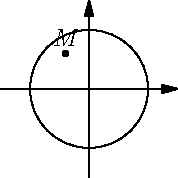
\includegraphics{Ectrigus90_1.pdf}
 \caption{Exercice Ectrigus90}
 \label{fig:Ectrigus90_1}
\end{figure}
